% Chapter 1

\chapter{Desarrollo} % Main chapter title

\label{Chapter1} % For referencing the chapter elsewhere, use \ref{Chapter1} 
\label{IntroGeneral}

%----------------------------------------------------------------------------------------

% Define some commands to keep the formatting separated from the content 
\newcommand{\keyword}[1]{\textbf{#1}}
\newcommand{\tabhead}[1]{\textbf{#1}}
\newcommand{\code}[1]{\texttt{#1}}
\newcommand{\file}[1]{\texttt{\bfseries#1}}
\newcommand{\option}[1]{\texttt{\itshape#1}}
\newcommand{\grados}{$^{\circ}$}

%----------------------------------------------------------------------------------------

%\section{Introducción}

%----------------------------------------------------------------------------------------
\section{Introducción}

En el presente trabajo práctico, se desarrolla la implementación del algoritmo Monte Carlo ES en un modelo que, luego de ser entrenado, es capaz de jugar al tres en linea. El objetivo es poder evaluar la implementación del algoritmo, sus beneficios y defectos, y también su rendimiento en un juego simple y reducido.

Para lograrlo, se implementaron en lenguaje Python las clases \textit{Board}, y \textit{TicTacToe} que modelan el tablero y las reglas de juego respectivamente (entorno) ,y la clase abstracta \textit{Player} que da soporte a las operaciones de los posibles jugadores (agentes). Heredando de \textit{Player}, se crearon las clases \textit{UserPlayer}, \textit{BotPlayer} y  \textit{MonteCarloEsControl} que permiten jugadores humanos, bots aleatorios y bots guiados por el algoritmo de Monte Carlo ES respectivamente.

Un script principal facilita la ejecución de los casos de uso principales: comenzar un juego entre 2 jugadores o entrenar un agente de Monte Carlo.

\section{Entorno}

El juego comienza luego de definir 2 tipos de jugadores entre las 3 posibilidades, instanciar la clase \textit{TicTacToe} y ejecutar el método \textit{start}. En ese instante se imprime en pantalla un tablero de tres en línea como se muestra en la figura \ref{fig:board}. 

\begin{figure}[htbp]
	\centering
	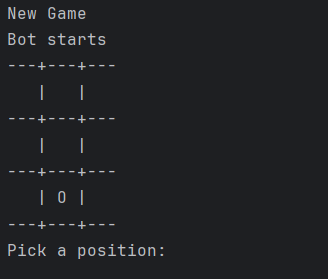
\includegraphics[width=.5\textwidth]{./Figures/board.png}
	\caption{Tablero de tres en linea.}
	\label{fig:board}
\end{figure}

El comportamiento inicial dependerá de los jugadores seleccionados como jugador 1 y 2 y del azar, que le asignará a cualquiera de los anteriores la jugada inicial. Cada vez que un jugador realice una jugada valida, el tablero se refrescará y la partida continuará hasta que haya un ganador o se produzca un empate (tablero lleno). En este momento se detiene el juego y se informa el resultado, como se muestra en la figura \ref{fig:board_end}.

\begin{figure}[htbp]
	\centering
	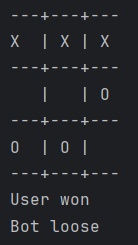
\includegraphics[width=.25\textwidth]{./Figures/board_end.png}
	\caption{Juego finalizado.}
	\label{fig:board_end}
\end{figure}

\section{Agentes}

Cuando  un jugador es humano y le llega su turno, este debe introducir por teclado un número del 0 al 8, correspondientes a las posiciones que se muestran en la figura \ref{fig:human_board}. Si el jugador ingresa una posición inválida o una posición ya tomada, se deberá volver a introducir la jugada.

\begin{figure}[htbp]
	\centering
	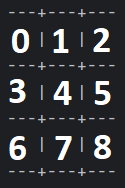
\includegraphics[width=.25\textwidth]{./Figures/human_board.png}
	\caption{Posiciones en el tablero.}
	\label{fig:human_board}
\end{figure}

El bot aleatorio elige, en forma automática y aleatoria, cualquier posición disponible en el tablero. Este no sigue ninguna estrategia y resulta útil únicamente para probar el juego y para realizar el entrenamiento del agente de Monte Carlo.

El agente de Monte Carlo realiza movimientos en forma automática siguiendo una política aprendida. En cada turno observa el estado actual del tablero, y toma la acción que se evaluó como mejor opción para ese estado durante el entrenamiento.

\section{Entrenamiento}

Para entrenar el agente de Monte Carlo, se ejecutaron múltiples juegos consecutivos de tres en línea donde participaban el agente en entrenamiento y bots aleatorios. Dentro del agente de Monte Carlo se implementó el algoritmo de la figura \ref{fig:algorithm}, con los siguientes detalles:
\begin{itemize}
    \item \(A(s)\) contiene las acciones posibles que son jugar las posiciones del 0 al 8.
    \item S contiene los estados posibles del tablero. El tablero de tres en línea tiene en total \(3^9 = 19.683\) estados diferentes, la mayoría de los cuales son ilegales.
    \item  Dado que resulta costoso generar las políticas para todos los estados del tablero y también filtrar solo los estados posibles (alrededor de 5.478), se decidió comenzar con \(\pi(s)\) y \(Q(s,a)\) vacíos e inicializarlos en forma aleatoria a medida que el agente se encontraba con estados que nunca había visto antes.
    \item Para el comienzo exploratorio de Monte Carlo, se ejecutaron en el tablero un número aleatorio de jugadas aleatorias alternadas entre jugador 1 y 2 previo a comenzar el episodio. Cabe destacar que se realizó un chequeo del estado del tablero luego de estas inicializaciones para verificar la validez.
    \item Como recompensa se asignó -0.1 por cada jugada que no concluyera en el final del juego, -10 a una jugada perdedora, -2 a una jugada de empate y 10 a una jugada ganadora.
    \item Adicionalmente se limito el número de jugadas del agente en 20 y se agrego una penalización de -50 si se supera este valor. De esta forma se prioriza que aprenda a jugar posiciones válidas.
    \item Se fijo un factor de descuento de 0.9.
    \item El entrenamiento se repitió durante 500.000 episodios, demorando aproximadamente una hora.
    \item Los valores anteriores se obtuvieron en forma empírica, a partir de varios entrenamientos y analizando los resultados obtenidos.
\end{itemize} 

\begin{figure}[htbp]
	\centering
	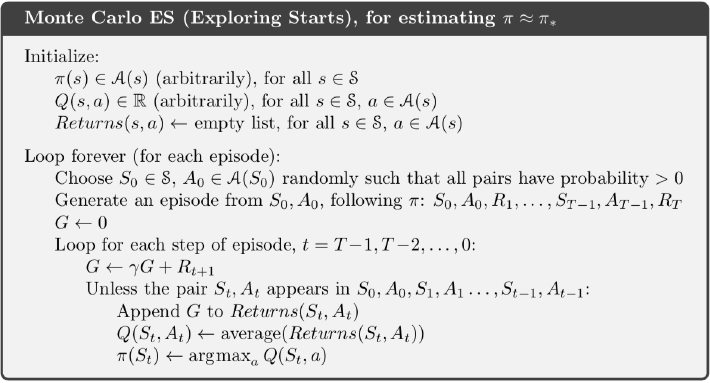
\includegraphics[width=0.8\textwidth]{./Figures/algorithm.png}
	\caption{Algoritmo de Mote Carlo ES.}
	\label{fig:algorithm}
\end{figure}

\section{Resultados}

Luego de entrenar el agente Monte Carlo ES durante 500.000 episodios se obtuvo un modelo capaz de identificar las estrategias principales del tres en línea. Por ejemplo, si el agente comienza el juego, este toma siempre el centro del tablero como se observa en la figura \ref{fig:monte_carlo_center}. También, si el agente tiene posibilidad de ganar, toma la posición ganadora; o por el contrario, si el contrincante tiene posibilidad de ganar, el agente intenta bloquear esa posibilidad, como se observa en las figuras \ref{fig:monte_carlo_win} y \ref{fig:monte_carlo_block}.

\begin{figure}[htbp]
	\centering
	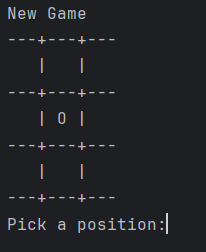
\includegraphics[width=0.25\textwidth]{./Figures/monte_carlo_center.png}
	\caption{Agente tomando el centro.}
	\label{fig:monte_carlo_center}
\end{figure}

\begin{figure}[htbp]
	\centering
	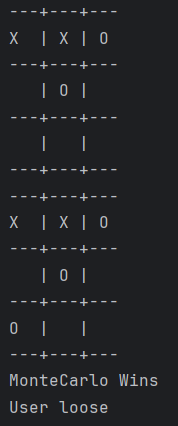
\includegraphics[width=0.25\textwidth]{./Figures/monte_carlo_win.png}
	\caption{Agente tomando la posición ganadora.}
	\label{fig:monte_carlo_win}
\end{figure}

\begin{figure}[htbp]
	\centering
	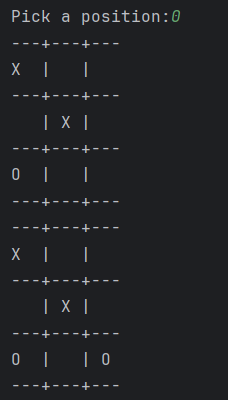
\includegraphics[width=0.25\textwidth]{./Figures/monte_carlo_block.png}
	\caption{Agente bloqueando la posición ganadora del humano.}
	\label{fig:monte_carlo_block}
\end{figure}

Lo sorprendente es que el agente también aprende estrategias avanzadas, Por ejemplo, si teniendo tomado el centro el usuario elije posición 1, 3, 5 o 7, la victoria esta asegurada con el patrón de la figura \ref{fig:monte_carlo_advanced}. A la vez, si el jugador intenta ejecutar la misma estrategia sobre el agente, este la evita eligiendo las esquinas como su primer movimiento.

\begin{figure}[htbp]
	\centering
	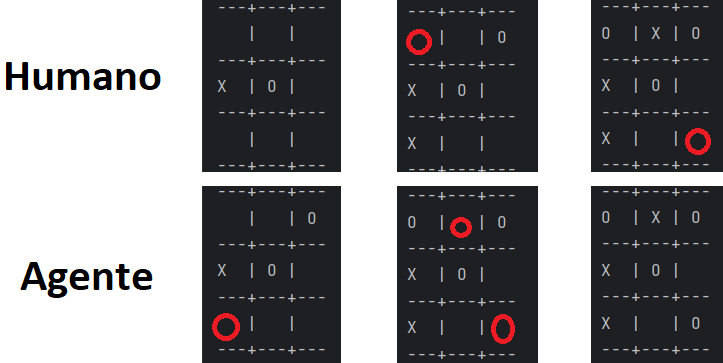
\includegraphics[width=\textwidth]{./Figures/monte_carlo_advanced.png}
	\caption{Agente ejecutando estrategia que asegura la victoria. En rojo posiciones ganadoras.}
	\label{fig:monte_carlo_advanced}
\end{figure}

Como contrapartida el agente no es perfecto, cuando se intenta ejecutar sobre el mismo otra estrategia ganadora mostrada en la figura \ref{fig:monte_carlo_exception}, este falla eligiendo repetidamente una posición ya tomada. Esto se debe a que en el entrenamiento no se exploró el espacio de estados y acciones lo suficiente como para encontrar una mejor política.

\begin{figure}[htbp]
	\centering
	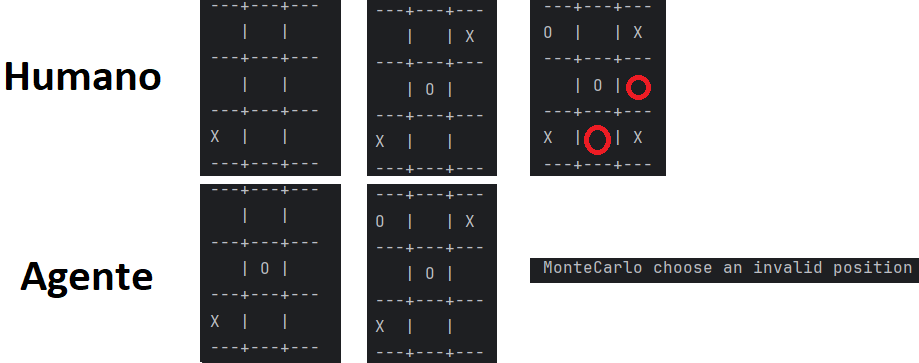
\includegraphics[width=\textwidth]{./Figures/monte_carlo_exception.png}
	\caption{Agente fallando en tomar posiciones válidas.}
	\label{fig:monte_carlo_exception}
\end{figure}

\section{Futura mejoras}

Como futura mejora se plantea crear una clase \textit{Trainer} que agregue visualizaciones de métricas útiles durante el entrenamiento como el valor Q medio de todos los estados cada cierto número de episodios, o la cantidad de victorias, pérdidas y empates logrados en los últimos 100 episodios.

\section{Conclusiones}

El algoritmo mostró resultados muy buenos en el desafío planteado, no solamente aprendiendo los movimientos básicos, sino también aprendiendo estrategias avanzadas lo cual es inesperado dada la sencillez del algoritmo. Como puntos débiles, aún en un juego simple como el tres en línea, se deben mantener estructuras para todos los estados posibles del tablero (que en este caso es del orden de los miles) lo que requiere de un entrenamiento de muchos episodios (en el orden del millón), haciéndolo lento. Otro punto débil del algoritmo es que debido que el algoritmo no puede ``extrapolar`` conocimiento, es decir aprovechar lo aprendido para un estado para resolver estados similares.